\documentclass[letterpaper, 12pt]{article}
\usepackage[utf8]{inputenc}
\usepackage[german]{babel} %no se si es ngerman o german en diferentes paginas es uno y en otra otro
%--------------------------------
%Paqueterias

\usepackage[left=1cm, right=2cm,top=2cm,foot=1cm]{geometry}
\usepackage{graphicx}
\usepackage{amsmath} 
\usepackage{amssymb}
\usepackage{mathrsfs}
\usepackage{latexsym}
\usepackage{dsfont}
\usepackage[usenames,dvipdsnames,svgnames,x11names]{xcolor}
\usepackage{enumerate}
\usepackage{enumitem}
\usepackage{array}
\usepackage{multirow}
%\usepackage{thebibliography}
\usepackage[style=apa]{biblatex}%para poner las cosas con nombre de autor etc, ejemplo:[backend=biber, citestyle =alphabetic, style=apa]
\bibliography{bio}
\usepackage{fancyhdr}
\usepackage{hyperref}
%----------------------------------------------------
%Encabezado y pie de pagina 
\pagestyle{fancy}
\fancyhf{}
\lhead{\leftmark}
\lfoot{Valencia Sánchez Francisco David}
\rfoot{\thepage}

%--------------------------------------------------
\begin{document}
{{{\large{\textls{\textbf{{{\textcolor{ForestGreen}{{Ecuaciones para la vida}}}}}}}}}\\
{{\large{{\textcolor{Maroon}{Valencia Sánchez Francisco David}}}}\\ 
\normalsize{\textcolor{Brown}{27 Octubre 2022}}}\\}
%---------------------------------------------

\section{Problemas}
    
    %-------------- Probelama 1 --------------------------

\begin{enumerate}

\item {{Considerando un sistema en una dimensión y sabiendo que $a=\frac{dv}{dt}$ y $v=\frac{dx}{dt}$ Demuestre que la posición se puede ver como:}}
    \begin{equation}
    \label{Ecuación de posición en el eje x}
        x=x_0 + v_0 t + \frac{1}{2} at^2
    \end{equation}
Para un tiempó inicial $t= 0 $ y con; $x_0$ y $v_0 $ la posición y la velocidad inicial en el sistema.\\
Sabemos que 
\begin{equation}
    v=\frac{dx}{dt}
\end{equation}
Sacamos la integral 
\begin {equation}
\int_{0} ^{t} a = dt = \int_{v_0}^{v} dv
\end{equation}
Definimos la integral
\begin {equation}
at |_{0}^{t} = v |_{v_0}^{v} 
\end{equation}

\begin {equation}
at – a(0) = v – v_0
\end{equation}
Nos queda:
\begin{equation}
at = v – v_0
\end{equation}

Por lo que tenemos:
\begin{equation}
\label{Eq de velocidad}
v = v_0 + at 
\end{equation}

Una vez demostrado esta primera parte, lo que es la velocidad, podemos empezar a definir la siguiente afirmación:

\begin{equation} 
v dt = dx 
\end{equation}
Sabemos que en la ecuación \ref{Eq de velocidad} nos da la velocidad por lo que sustituimos 
\begin{equation} 
(v_0 + at) dt = dx 
\end{equation}
Integramos 
\begin{equation} 
\int_{0} ^{t} (v_0 + at) dt =  _{x_0} ^{x} dx 
\end{equation}
Definimos la integral
\begin{equation}
v_0 t + \frac{at^2}{2} |_{0}^{t} = x |_{x_0}^{x}
\end{equation}
Nos queda 
\begin{equation}
v_0 t + \frac{1}{2} at^2 = x – x_0
\end{equation}

Por lo que tenemos la fórmula de movimiento en el eje x 

\begin{equation}
x = x_0 + v_0 t + \frac{1}{2} at^2 
\end{equation}

Quedo Demostrado 


    %--------------------- Problema 2 -----------------------
    
    \item Considere una carrera entre dos coches estos arrancan del reposo pero el coche uno hace trampa (cosa que nunca pasa), saliendo un segundo amtes que el segundo, si los autos tienen una aceleración de $3.5 m/s^2$  y  $4.9 m/s^2$ respectivamente.
    
\begin{enumerate}
    \item {En que momento el auto dos alcanza al auto uno i.e $t=?$}\\
Tenemos la formula que acabamos de demostrar \ref{Ecuación de posición en el eje x} podemos empezar a definir algunos datos que tenemos:\\
Ambos han recorrido la misma distancia, por lo que ambas son igual a x, ademas que la distancia inicial sera de 0 asi como su velocidad inicial.\\
En el escrito nos dice que se adelanta 1 segundo por lo que el tiempo real seria el siguiente para el auto 1.\\
El auto 2 tiene una aceleración de $3.5m/s^2$
\begin{equation}
\label{Ecuacion inciso a auto 1}
    x= \frac{1}{2} a_{a1} t^2 
\end{equation}
\begin{equation}
\label{Ecuación inciso a auto 2}
     x= \frac{1}{2} (3.5 m/s^2)(t-1s)^2 
\end{equation}
\\
El auto 1 tiene una aceleración de $4.9m/s^2$
Mientras que el tiempo del auto 1 es:\\
\begin{equation}
    x = \frac{1}{2} a_{a2}t^2
\end{equation}
\begin{equation}
    x = \frac{1}{2} (4.9 m/s^2)t^2
\end{equation}
\\
Igualamos las dos ecuaciones que nos dieron ya que al recorrer la misma distancia tienen la misma x.

\begin{equation}
\label{Eq inciso 2 ya igualada}
    \frac{1}{2} (3.5 m/s^2)(t-1s)^2 = \frac{1}{2} (4.9 m/s^2)t^2
\end{equation}
Multipicamos y vamos desarrollando el binomio que se encuentra ahí, el objetivo es reducirla a un estado en el que podamos encontrar la t, ya que es la variable que deseamos conocer.
\begin{equation}
    \frac{3.5}{2} (t^2 - 2t + 1) = \frac{4.9}{2} t^2
\end{equation}
\begin{equation}
    \frac{3.5t^2 - 7t + 3.5}{2} = \frac{4.9}{2} t^2
\end{equation}
\begin{equation}
    (2)(\frac{3.5t^2 - 7t + 3.5}{2}) = 4.9t^2
\end{equation}
\begin{equation}
    3.5t^2 - 7t + 3.5 = 4.9t^2
\end{equation}
Igualamos a 0 para poder tener una ecuación normal de segundo grado
\begin{equation}
    3.5t^2 - 7t + 3.5 - 4.9t^2 = 0
\end{equation}
\begin{equation}
    -1.4t^2 - 7t + 3.5  = 0
\end{equation}
Por nuestra comodidad y para la del lector pasaremos de decimales a fraccionarios para poder manejar mejor los números vemos que tiene multiplo el cual es 10.
\begin{equation}
    -\frac{7}{5}t^2 - 7t + \frac{7}{2}  = 0
\end{equation}
\begin{equation}
    2t^2 + 10t -5 = 0
\end{equation}
Una vez igualada a 0 podemos resolverla por la formula general la cual es 
\begin{equation}
     x = \frac{-b \pm \sqrt{b^2 - 4ac}}{2a}
\end{equation}
Sustituimos los valores en la formula y vamos desarrollando
\begin{equation}
    t = \frac{- 10 \pm \sqrt{-10^2 - 4(2)(-5)}}{2(2)}
\end{equation}
\begin{equation}
    t = \frac{- 10 \pm \sqrt{100+40}}{4}
\end{equation}
\begin{equation}
    t = \frac{- 10 \pm \sqrt{140}}{4}
\end{equation}
Como es cuadratica tenemos dos t por lo que $t_1$
\begin{equation}
    t_1 = \frac{- 10 - \sqrt{140}}{4}
\end{equation}
\begin{equation}
\label{Ecuacion t_1 del inciso a}
    t_1 = -5.45804
\end{equation}
Mientras que $t_2$
\begin{equation}
    t_2 = \frac{- 10 + \sqrt{140}}{4}
\end{equation}
\begin{equation}
    t_2 = 0.4504
\end{equation}
Es claro y evidente que el resultado que se parece más a la realidad es el de la ecuacion \ref{Ecuacion t_1 del inciso a}\\
Por lo que podemos decir y concluir que el tiempo en que el auto tarda en alcanzarlo es de -5.45 segundos .

    \item Cuál será la posición cuando el inciso (a) ocurra $x=?$\\
Para poder responder esta pregunta es muy facil ya que solo debemos sustituir los valores que ya tenemos en la ecuación \ref{Ecuación de posición en el eje x}, recordando que el auto se adelanto 1 segundo, y esto lo tomamos en cuenta al sacar el tiempo en la ecuación \ref{Ecuacion inciso a auto 1}
    \begin{equation}
    x=x_0 + v_0 t + \frac{1}{2} at^2
    \end{equation}
Sustituimos y nos queda:
    \begin{equation}
    x= \frac{1}{2} (3.5m/s^2)(5.45+1)^2
    \end{equation}
El resultado es:
\begin{equation}
    72.9859m
\end{equation}
Para que quede aun mas claro (\textbf{\textcolor{red}{Ya que la forma en la que se redacto el problema es un poco confusa}}) ahora lo haremos con la ecuación \ref{Ecuación inciso a auto 2} a la cual ya no le tenemos que sumar 1
Sustituimos y nos queda:
    \begin{equation}
    x= \frac{1}{2} (4.9m/s^2)(5.45)^2
    \end{equation}
El resultado es:
\begin{equation}
    72.9859m
\end{equation}
Nos da el mismo resultado por lo que, quedo resuelto este segundo inciso.

    \item Cuál será la velocidad que tendrá en ese punto para ambos autos
    
Sabemos que la Velocidad con aceleración de 4.90$m/s^2$es:
\begin{equation}
    v = a_1 t
\end{equation}
\begin{equation}
    v = (4.90m/s^2)(5.45s)
\end{equation}
\begin{equation}
    v = 26.8 m/s
\end{equation}
Por lo tanto la velocidad en el auto con la aceleración de 3.5$m/s^2$es:
\begin{equation}
\label{Ecuación v}
    v = a_2 t
\end{equation}
\begin{equation}
    v = (3.5m/s^2)(6.45s)
\end{equation}
\begin{equation}
    v = 22.6 m/s
\end{equation}


    \item Toma 5 tiempos diferentes a partir de que los autos arrancan, sin tomar el tiempo inicial, 3 antes del tiempo donde los autos se encuentran y dos posteriores a ese tiempo, realicen dos tablas, una para cada auto, con la siguiente información; aceleración, tiempo posición y velocidad.\\

    
    %--------------------  Tabla 1 ---------------------
 \begin{table}[h]
\label{Tabla de 3.5)}
    \centering
\caption{{Cinemática del Auto con Aceleración 3.5$m/s^2$}}

\begin{tabular}{c|c|c|c|c|c} \hline \hline
\multicolumn{6}{c}{Auto con Aceleración 3.5$m/s^2$}\\\hline 
\multicolumn{3}{c|}{No dependiente del tiempo} & \multicolumn{3}{c}{Dependientes del tiempo}\\\hline
\multicolumn{3}{c|} {$a[m/s^2]$} & $t[s]$ & $x[m]$ & $v[m/s$  \\ \hline
\multicolumn{3}{c|}{} &7.45s  &97.12m &26.075m/s \\\cline{4-6}
\multicolumn{3}{c|}{} &8.45s  &124.95m &29.575m/s \\ \cline{4-6}
\multicolumn{3}{c|} {3.5$m/s^2$} &2.45s &10.50m &8.575m/s  \\ \cline{4-6}
\multicolumn{3}{c|}{} &3.45s  &20.82m &12.07m/s \\ \cline{4-6}
\multicolumn{3}{c|}{} &4.45s  &34.65m &15.57m/s\\ \hline \hline
\end{tabular}\\
  \end{table}
 
\vspace{2cm} 
A continuación las cuentas que hice para obtener los valores de la tabla \ref{Tabla de 3.5)}
Primero los dos tiempos posteriores, tomando en cuenta la ecuación \ref{Ecuación de posición en el eje x}\\
Tiempo 7.45s sustituimos y nos queda:
    \begin{equation}
    x= \frac{1}{2} (3.5m/s^2)(7.45)^2 = 97.12m
    \end{equation} 
La velocidad es de, tomando en cuenta la ecuación \ref{Ecuación v}
\begin{equation}
    v = (3.5m/s^2)(7.45s) = 26.075m/s
\end{equation}
Tiempo 8.45s sustituimos y nos queda:
    \begin{equation}
    x= \frac{1}{2} (3.5m/s^2)(8.45)^2 = 124.95m
    \end{equation} 
La velocidad es de, tomando en cuenta la ecuación \ref{Ecuación v}
\begin{equation}
    v = (3.5m/s^2)(8.45s) = 29.575m/s
\end{equation}
Ahora los tiempos antes de alcanzarlo \\
Tiempo 2.45s sustituimos y nos queda:
    \begin{equation}
    x= \frac{1}{2} (3.5m/s^2)(2.45s)^2 = 10.50m
    \end{equation} 
La velocidad es de, tomando en cuenta la ecuación \ref{Ecuación v}
\begin{equation}
    v = (3.5m/s^2)(2.45s) = 8.575m/s
    \end{equation}
Tiempo 3.45s sustituimos y nos queda:
    \begin{equation}
    x= \frac{1}{2} (3.5m/s^2)(3.45s)^2 = 20.82m
    \end{equation} 
La velocidad es de, tomando en cuenta la ecuación \ref{Ecuación v}
\begin{equation}
    v = (3.5m/s^2)(3.45s) = 12.07m/s
    \end{equation}
Tiempo 4.45s sustituimos y nos queda:
    \begin{equation}
    x= \frac{1}{2} (3.5m/s^2)(4.45s)^2 = 34.65m
    \end{equation} 
La velocidad es de, tomando en cuenta la ecuación \ref{Ecuación v}
\begin{equation}
    v = (3.5m/s^2)(4.45s) = 15.57m/s
    \end{equation}
\end{enumerate}
\\
\vspace{1cm}
     %--------------------  Tabla 2 ---------------------
 \begin{table}[h]
\label{Tabla de auto 4.9}
    \centering
\caption{{Cinemática del Auto con aceleración 4.9$m/s^2$}}

\begin{tabular}{c|c|c|c|c|c} \hline \hline
\multicolumn{6}{c}{Auto con aceleración 4.9$m/s^2$}\\\hline 
\multicolumn{3}{c|}{No dependiente del tiempo} & \multicolumn{3}{c}{Dependientes del tiempo}\\\hline
\multicolumn{3}{c|} {$a[m/s^2]$} & $t[s]$ & $x[m]$ & $v[m/s$  \\ \hline
\multicolumn{3}{c|}{} &8.45s &174.93m &41.40m/s  \\\cline{4-6}
\multicolumn{3}{c|}{} &7.45s &135.98m &36.505m/s \\ \cline{4-6}
\multicolumn{3}{c|} {4.9$m/s$} &2.45s &14.70m &12.00m/s   \\ \cline{4-6}
\multicolumn{3}{c|}{} &3.45 &29.16m  &16.45m/s  \\ \cline{4-6}
\multicolumn{3}{c|}{} &4.45s &48.51m  &21.80m/s \\ \hline \hline
\end{tabular}\\
  \end{table}

 %------------------Cambiar valores 
 A continuación las cuentas que hice para obtener los valores de la tabla \ref{Tabla de auto 4.9}
Primero los dos tiempos posteriores, tomando en cuenta la ecuación \ref{Ecuación de posición en el eje x}\\
Tiempo 7.45s sustituimos y nos queda:
    \begin{equation}
    x= \frac{1}{2} (4.9m/s^2)(7.45)^2 = 135.98m
    \end{equation} 
La velocidad es de, tomando en cuenta la ecuación \ref{Ecuación v}
\begin{equation}
    v = (4.9m/s^2)(7.45s) = 36.505m/s
\end{equation}
Tiempo 8.45s sustituimos y nos queda:
    \begin{equation}
    x= \frac{1}{2} (4.9m/s^2)(8.45)^2 = 174.93m
    \end{equation} 
La velocidad es de, tomando en cuenta la ecuación \ref{Ecuación v}
\begin{equation}
    v = (4.9m/s^2)(8.45s) = 41.40m/s
\end{equation}
Ahora los tiempos antes de alcanzarlo \\
Tiempo 2.45s sustituimos y nos queda:
    \begin{equation}
    x= \frac{1}{2} (4.9m/s^2)(2.45s)^2 = 14.70m
    \end{equation} 
La velocidad es de, tomando en cuenta la ecuación \ref{Ecuación v}
\begin{equation}
    v = (4.9m/s^2)(2.45s) = 12.00m/s
    \end{equation}
Tiempo 3.45s sustituimos y nos queda:
    \begin{equation}
    x= \frac{1}{2} (4.9m/s^2)(3.45s)^2 = 29.16m
    \end{equation} 
La velocidad es de, tomando en cuenta la ecuación \ref{Ecuación v}
\begin{equation}
    v = (4.9m/s^2)(3.45s) = 16.45m/s
    \end{equation}
Tiempo 4.45s sustituimos y nos queda:
    \begin{equation}
    x= \frac{1}{2} (4.9m/s^2)(4.45s)^2 = 48.51m
    \end{equation} 
La velocidad es de, tomando en cuenta la ecuación \ref{Ecuación v}
\begin{equation}
    v = (4.9m/s^2)(4.45s) = 21.80m/s
    \end{equation}

\newpage
%------------------ Problema 3 -------------------------
    \item Considere el siguiente sistema, dos bloques de masas $m1$ y $m2$ estan unidos por una cuerda ideal y descansan sobre una superficie horizontal sin roce. Si una fuerza de magintud $A$ se le aplica al bloque de masa $m2$ horizontalmente, en la dirección que muestra la Figura 1. Realicen los respectivos diagramas de cuerpos libres (usen powerpoint, pait, dibújelo, lo que gusten) y anexelo   como una imagen, a partir de ellos determinen la aceleración del sistema y la tensión de la cuerda entre los bloques.\\

A continuación en la imagen se presenta el diagrama de cuerpo libre donde se reprentan de manera grafica las fuerzas que estan sobre los cuerpos de masa $m_1$ y $m_2$
Sabemos que la formula de la segunda ley de Newton 
\begin{equation}
\label{Eq Segunda ley}
    F = ma
\end{equation}
Observe que tenemos dos masas por lo que en la ecuación \ref{Eq Segunda ley}
vamos a sustituir la m por la suma de las dos masas
\begin{equation}
    F = (m_1 + m_2)a
\end{equation}
Entonces sabemos que la tensión $t - t$ seria $m_1 a$
Por lo tanto 
\begin{equation}
    T = (m_1 -m_2)a + A
\end{equation}

\end{enumerate}
    \begin{figure}
    \centering
        \caption{Diagrama de cuerpo libre }
    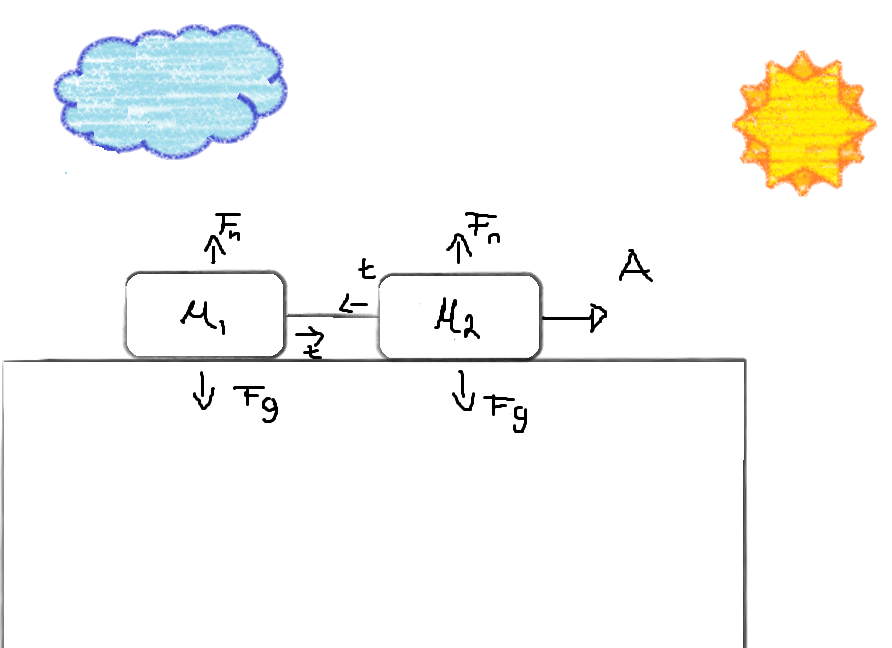
\includegraphics[scale=0.40]{Diagrama de cuerpo libre.png}

    \label{fig, diagrama}
\end{figure}

%----------------------------------------------------------
\section{Punto Extra}
\begin{itemize}
    \item Investigación del comando ¨hyperref"\\
    
Hacer un documento navegable es tan sencillo como cargar el paquete hyperref, automáticamente las referencias en el texto y la tabla de contenidos se convierten en“links”
que nos llevan hasta la referencia o la sección correspondiente. Puesto que el paquete
hyperref redefine muchos comandos LATEX es conveniente que sea el último paquete
en cargarse.
Para cargarlo, se utiliza la sintaxis habitual:
usepackage[opciones]{hyperref}\\
Este comando lo utilice para poder hacer referencias de una manera mas creativa, al tocar el numero de color rojo nos va dirigir a la ecuacion o imagen a la que estoy citando dentro del documento y asi no volver a escribir cada escuación de nuevo.
\end{itemize}

%-----------------------------------
\begin{thebibliography}{}
\bibitem{Holi}. (2022). Retrieved 6 November 2022, from https://mat.uda.cl/hsalinas/cursos/2008/latex/apuntes10.pdf

\end{thebibliography}

\end{document}
